\begin{frame}{Global Picture}
\centering
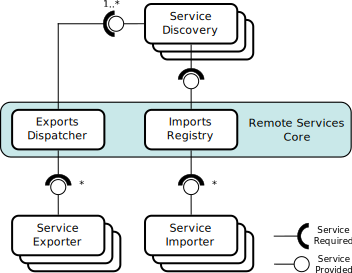
\includegraphics[height=.8\textheight]{../imgs/rs_arch}
\end{frame}

\begin{frame}{Remote Services: Public Services}
\begin{small}
\begin{exampleblock}{Note}
All services names are declared in \texttt{pelix.remote}
\end{exampleblock}

\begin{block}{Core Services}
\begin{itemize}
\item[] \texttt{RemoteServiceDispatcher}
\begin{itemize}
\vspace{-.5em}
\item[] Read-only access to the list of export endpoints
\end{itemize}
\item[] \texttt{RemoteServiceDispatcherServlet}
\begin{itemize}
\vspace{-.5em}
\item[] Utility methods for HTTP-based discovery
\end{itemize}
\item[] \texttt{RemoteServiceRegistry}
\begin{itemize}
\vspace{-.5em}
\item[] Write-only access to the list of import endpoints
\end{itemize}
\end{itemize}
\end{block}
\end{small}
\end{frame}

\begin{frame}{Remote Services: Providers Services}
\begin{small}
\begin{exampleblock}{Note}
All services names are declared in \texttt{pelix.remote}
\end{exampleblock}

\begin{block}{Import/Export Services}
\begin{itemize}
\item[] \texttt{RemoteServiceExportProvider}
\begin{itemize}
\item[] Notified by the dispatcher to create export endpoints
\end{itemize}
\item[] \texttt{RemoteServiceExportEndpointListener}
\begin{itemize}
\item[] Notified of new export endpoints
\end{itemize}
\item[] \texttt{RemoteServiceImportEndpointListener}
\begin{itemize}
\item[] Notified of new import endpoints
\end{itemize}
\end{itemize}
\end{block}
\end{small}
\end{frame}

\begin{frame}{Endpoint creation sequence}
\begin{small}
\begin{block}{Service export/import}
The \texttt{Dispatcher} is notified of a service to be exported (after its registration or update), notifies the exporters and notifies the discovery services about the created endpoints.
\end{block}
\end{small}

\vspace{2ex}

\centering
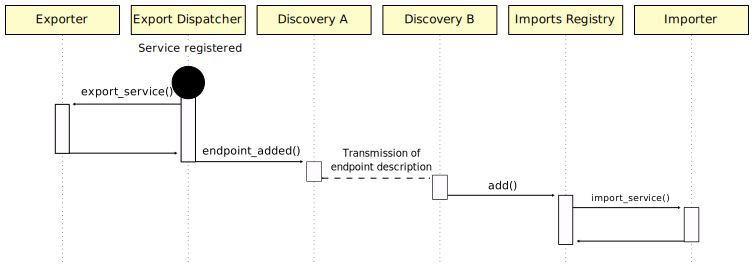
\includegraphics[width=\textwidth]{../imgs/rs_sequence}
\end{frame}

\begin{frame}{How to export a service?}
\begin{block}{How it works}
\begin{enumerate}
\item Services with export properties are detected by the dispatcher
\item The dispatcher notifies the export services
\item Each exporter can create an \texttt{ExportEndpoint}
\item The dispatcher notifies the discovery services
\end{enumerate}
\end{block}

\begin{block}{Export properties}
\begin{itemize}
\item[] \texttt{\small service.exported.interfaces}
\begin{itemize}
\vspace{-.2em}
\item[] List of exported interfaces
\end{itemize}
\item[] \texttt{\small service.exported.configs}
\begin{itemize}
\vspace{-.2em}
\item[] List of allowed export protocols
\end{itemize}
\end{itemize}
\end{block}
\end{frame}

\begin{frame}{How is a service imported?}
\begin{block}{How it works}
\begin{enumerate}
\item A discovery service detects a new service
\item The discovery service notifies the Imports Registry
\item The ImportRegistry notifies the import services
\item Each import service can register a proxy as a local service, with import properties
\end{enumerate}
\end{block}
\end{frame}

\begin{frame}{How is a service imported?}
\begin{block}{Imported service properties}
\begin{itemize}
\item[] \texttt{\small service.imported.interfaces}
\begin{itemize}
\vspace{-.2em}
\item[] List of exported interfaces
\end{itemize}
\item[] \texttt{\small service.imported.configs}
\begin{itemize}
\vspace{-.2em}
\item[] List of allowed export protocols
\end{itemize}
\item[] \texttt{\small endpoint.framework.uuid}
\begin{itemize}
\vspace{-.2em}
\item[] UUID of the host framework
\end{itemize}
\item[] \texttt{\small endpoint.service.id}
\begin{itemize}
\vspace{-.2em}
\item[] Service ID in the host framework
\end{itemize}
\end{itemize}
\end{block}
\end{frame}


\begin{frame}{Supported protocols}
\begin{exampleblock}{Java compatibility}
A Java implementation of iPOPO Remote Services is available as the \href{https://github.com/cohorte/cohorte-remote-services}{Cohorte Remote Services} project.
\end{exampleblock}

\begin{small}
\begin{columns}[t,onlytextwidth]
\column{.4\textwidth}
\begin{block}{Discovery}
\centering
\begin{tabular}{ll}
\textbf{Protocol} & \textbf{Specification}\\
Multicast & iPOPO\\
MQTT & iPOPO\\
ZeroConf & Standard\\
\end{tabular}
\end{block}

\column{.55\textwidth}
\begin{block}{Transport}
\centering
\begin{tabular}{ll}
\textbf{Protocol} & \textbf{Specification}\\
XML-RPC & Standard\\
JSON-RPC & Standard\\
Jabsorb-RPC & \href{https://code.google.com/archive/p/jabsorb/}{Jabsorb} project\\
MQTT-RPC & iPOPO \\
\end{tabular}
\end{block}
\end{columns}
\end{small}
\end{frame}
